\chapter{Isomorphic Theorems}

\section{Normal Subgroups}

\begin{definition}[Normal Subgroup]\index{normal subgroup}\label{def:normal-subgroup}
    Let $G$ be a group and $N$ be a subgroup. We say $N$ is a \term{normal subgroup} of $G$, denoted $N \triangleleft G$, if \[
        \forall g \in G, gN = Ng.
    \] Equivalently, if $gNg^{-1} = N$. 
\end{definition}

\begin{definition}[Simple Group]\index{simple group}\label{def:simple-group}
    A group $G$ is \term{simple} if it has no nontrivial normal subgroups.
\end{definition}

\begin{example}
    Kernels of group homomorphisms are normal subgroups.

    \begin{proof}
        Let $x \in \ker{\phi}$ for some homomorphism $\phi: G \to H$. 
        
        Then, $\phi(gxg^{-1}) = \phi(g)\phi(x)\phi(g)^{-1} = \phi(g)e\phi(g)^{-1} = e$.
        
        Therefore, $gxg^{-1} \in \ker{\phi}$.
    \end{proof}
\end{example}

It is important to note that some group are normal under one group but not under another.

\begin{example}
    The alternating group, $A_n$, is normal in the symmetric group, $S_n$.

    This is because $A_n$ is the kernel of the sign homomorphism, which is a normal subgroup by the previous example.

    {~~~}

    For example, consider $S_3$ and $A_3$. \[
        S_3 = \{e, (12), (13), (23), (123), (132)\}, \quad A_3 = \{e, (123), (132)\}.
    \]

    We have $(13)A_3(13) = \{
        (13)e(13), (13)(123)(13), (13)(132)(13)
    \} = \{ 
        e, (132), (123) 
    \} = A_3$.
\end{example}

\section{The First Two Isomorphism Theorem}

\begin{definition}[Quotient Group]\index{quotient group}\label{def:quotient-group}
    Let $G$ be a group and $N$ a normal subgroup. Then, we can define the \term{quotient group} $G/N$ as the set of left cosets of $N$ in $G$ with the operation \[
        (gN)(hN) := (gh)N.
    \]
\end{definition}

% \begin{proof}
%     WTS $(gh)N$ is a group. 

%     \begin{enumerate}
%         \item \textbf{Closure:} Let $g_1N, g_2N \in G/N$. Then, \[
%             (g_1N)(g_2N) = (g_1g_2)N \in G/N.
%         \]
%         \item \textbf{Associativity:} Let $g_1N, g_2N, g_3N \in G/N$. Then, \[
%             (g_1N)((g_2N)(g_3N)) = (g_1N)(g_2g_3)N = (g_1g_2g_3)N = (g_1g_2)g_3N = ((g_1N)(g_2N))(g_3N).
%         \]
%         \item \textbf{Identity:} Let $eN \in G/N$. Then, \[
%             (gN)(eN) = (ge)N = gN = (eg)N = (eN)(gN).
%         \]
%         \item \textbf{Inverses:} Let $gN \in G/N$. Then, \[
%             (gN)(g^{-1}N) = (gg^{-1})N = eN = (g^{-1}g)N = (g^{-1}N)(gN).
%         \]
%     \end{enumerate}
% \end{proof}

\begin{theorem}
    $G/N$ is a group if and only if $N \triangleleft G$.
\end{theorem}

\begin{example}
    $A_n$ is normal in $S_n$, so $S_n/A_n$ is a group.

    $A_n$ has $2$ cosets: itself, and the set of all odd permutations. Therefore, $S_n/A_n \cong \Z_2$.

    \begin{center}
        \begin{tabular}{c|c|c}
                      & $A_n$     & $(12)A_n$ \\ \hline
            $A_n$     & $A_n$     & $(12)A_n$ \\ \hline
            $(12)A_n$ & $(12)A_n$ & $A_n$
        \end{tabular}
        $\quad \cong \quad$
        \begin{tabular}{c|c|c}
                & $0$ & $1$ \\ \hline
            $0$ & $0$ & $1$ \\ \hline
            $1$ & $1$ & $0$
        \end{tabular}
    \end{center}

    We have $S_n/A_n \cong \Z/2\Z = \{ 0, 1 \} = \{ -1, 1 \}$.
    
    Moreover, since $\sgn: S_n \to \{ -1, 1 \}$, we see $S_n/\ker{\sgn} \cong \im{\sgn}$. 
\end{example}

\begin{theorem}[The First Isomorphism Theorem]\index{first isomorphism theorem}\label{thm:first-isomorphism}
    Let $G$ be a group, and $\phi: G \to H$ be an homomorphism. Then, \[
        G/\ker{\phi} \cong \im{\phi}.
    \] and the isomorphism is given by \[
        \begin{matrix}
            G/\ker{\phi} & \to & \im{\phi} \\
            g\ker{\phi} & \mapsto & \phi(g)
        \end{matrix}
    \]
\end{theorem}

\begin{theorem}[The Correspondence Theorem]\index{correspondence theorem}\label{thm:correspondence}
    Let $G$ be a group, and $N \triangleleft G$. Then, there is a correspondence between the set of subgroups of $G$ containing $N$ and the set of subgroups of $G/N$. \[
        \begin{matrix}
            \left\{ H \le G \mid N \subseteq H \subseteq G \right\} & \longleftrightarrow & \{ K \le G/N \} \\
            H & \longleftrightarrow & H/N
        \end{matrix}
    \]
\end{theorem}

\begin{figure}[ht!]
    \centering

    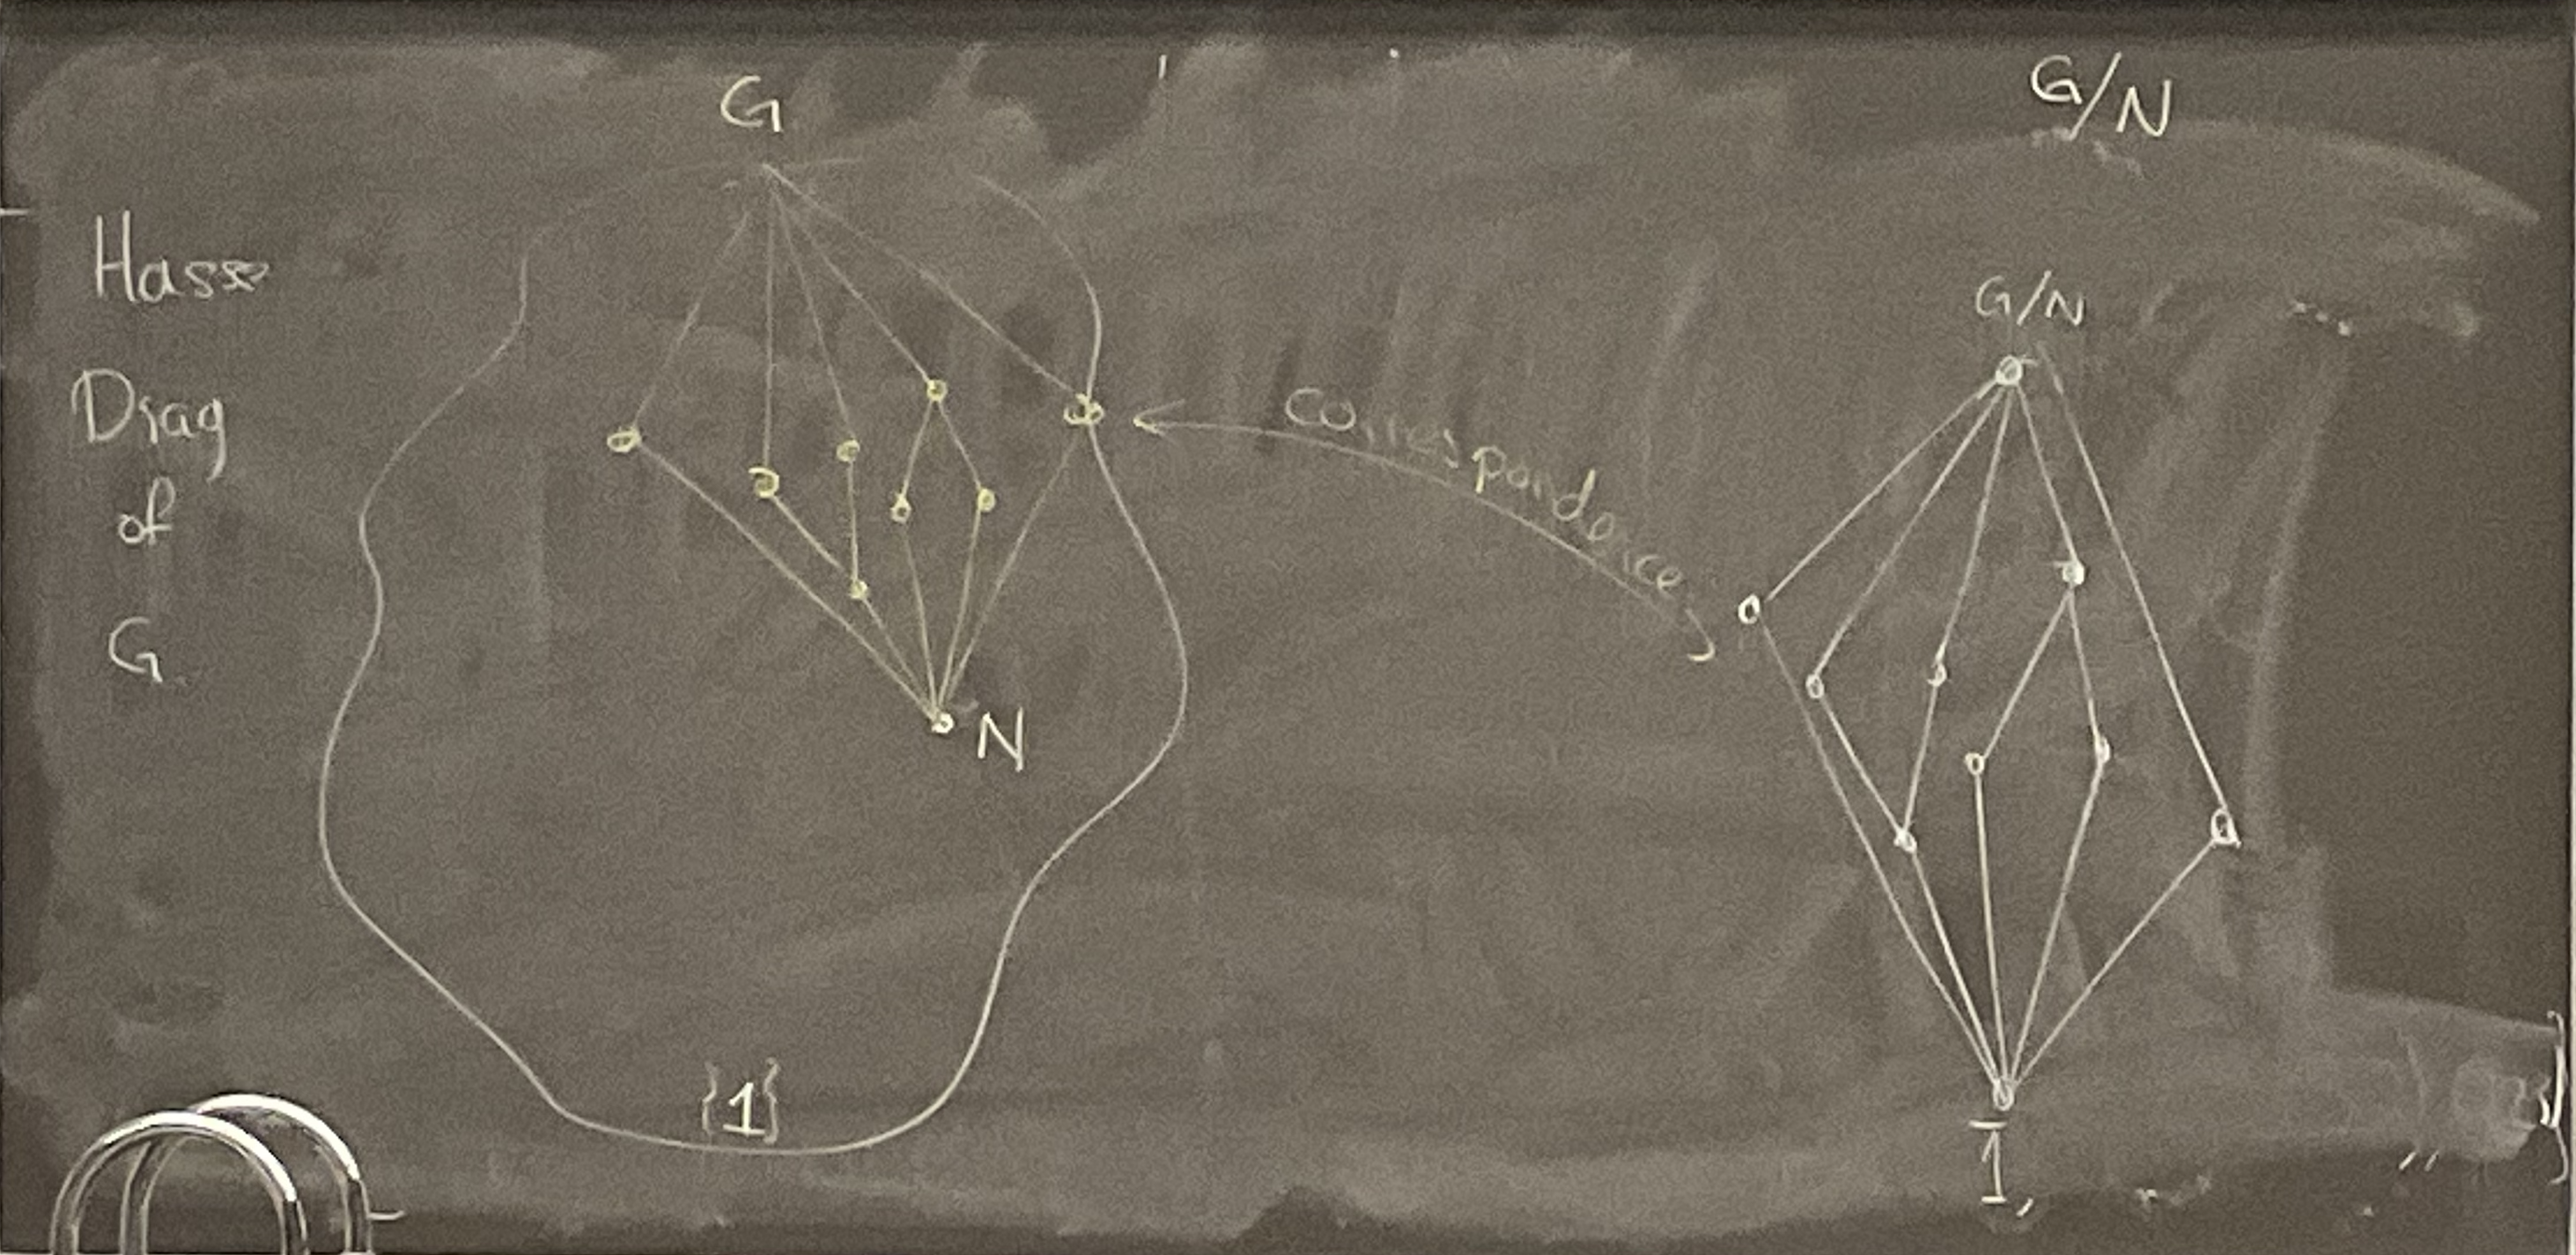
\includegraphics[width=0.67\linewidth]{figures/correspondence-theorem.png}
\end{figure}

The first isomorphism theorem tells us how to reduce the complexity of the group, and the correspondence theorem tells us that we do not loose any information when we do so.